
\chapter{Modellierung}\label{sec:chapter3}
Kapitel 3 liefert einen Überblick über die Grundlagen der Modellierung. Zunächst werden in Kapitel 3.1 die Grundlagen der Prozessmodellierung vorgestellt. Hierbei wird auf die Grundsätze ordnungsgemäßer Modellierung eingegangen. Anschließend werden in Kapitel 3.2 Prozessmodellierugssprachen vorgestellt. Einerseits wird hier auf imperative Modellierungssprachen eingegangen und es wird ein kurzer Einblick in die Prozessmodellierungssprache BPMN gegeben.Andererseits werden deklarative Prozessmodellierungssprachen vorgestellt und es erfolgt ein detaillierter Einblick in die deklarative Prozessmodellierungssprache ConDec.

\section{Prozessmodellierung}\label{sec:chapter3:Prozessmodellierung}

Prozessmodellierung hat den Zweck, Prozesse zu beschreiben \cite{fahland2009}. Ein Prozessmodell ist eine vereinfachte Darstellung eines Prozesses und besteht aus einer Abfolge von Tätigkeiten, welche chronologisch-sachlogisch angeordnet sind. Der Umfang und Detaillierungsgrad der Prozessmodelle kann sich je nach Zweck und Zielsetzung unterscheiden \cite{koch2011}.

\subsection{Ziele der Prozessmodellierung}
Mit der Modellierung von Prozessen werden verschiedene Ziele verfolgt. Eine erste Übersicht über die Ziele der Prozessmodellierung gibt Abbildung \ref{fig:ZieleProzess}.
\begin{figure}[htp]
\begin{center}
  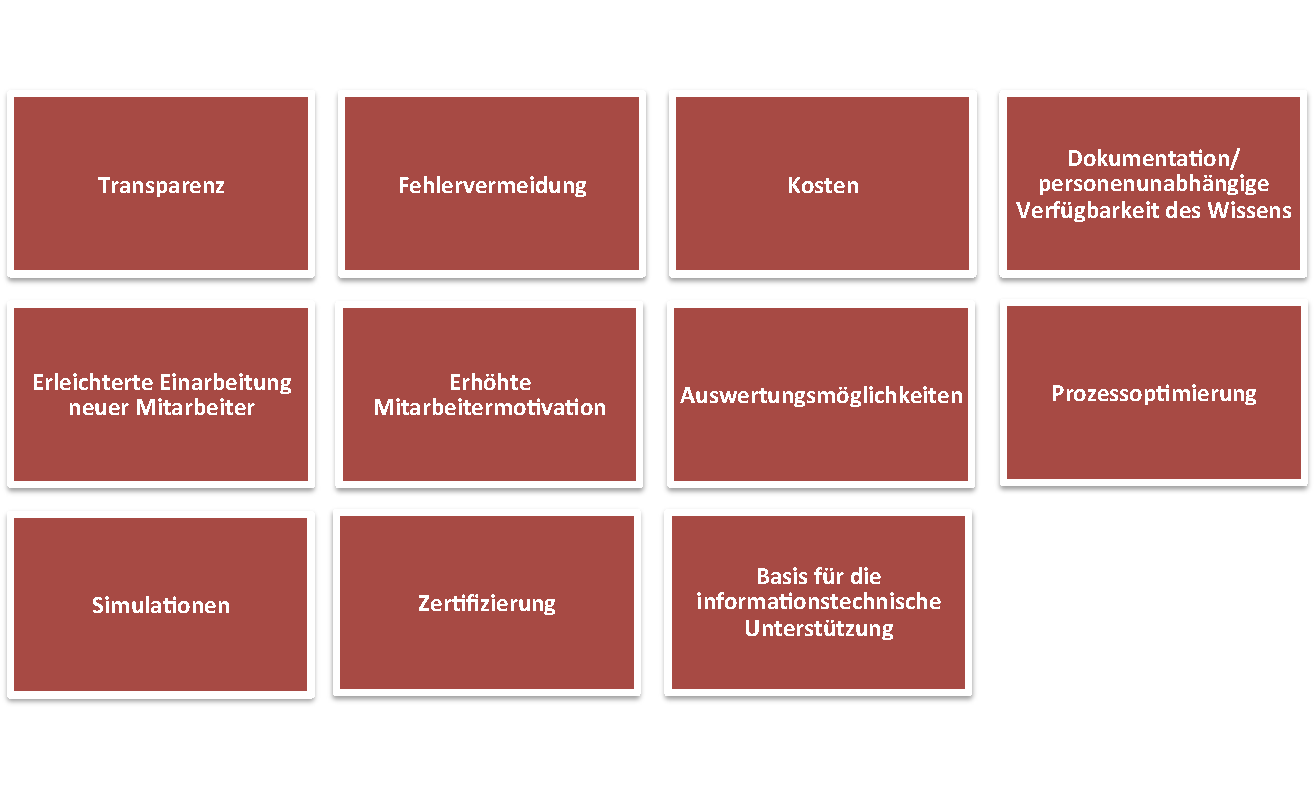
\includegraphics[scale=0.5]{ZieleProzess} %pdf, jpg, png...
  \caption{Ziele der Prozessmodellierung nach \cite{koch2011}}
  \label{fig:ZieleProzess}
\end{center}
\end{figure}

Bei der \textit{Transparenz} geht es darum, dass alle Beteiligten am Prozess einsehen können, von wem welche Aufgaben durchgeführt werden. Weiterhin verfolgt die Prozessmodellierung das Ziel, durch \textit{Fehlervermeidung} die Qualität, Termintreue und Kundenzufriedenheit zu erhöhen. Durch die Modellierung eines Prozesses kann dieser genau analysiert werden und hierdurch können Einsparungspotenziale von \textit{Kosten} aufgedeckt werden. Indem die Abläufe in einem Unternehmen als Prozesse dargestellt werden, ist es möglich eine \textit{personenunabhängige Verfügbarkeit des Wissens} zu erreichen, da das Wissen hierdurch allen Personen zugänglich gemacht wird, unabhängig davon, ob sie am Prozess beteiligt sind oder nicht. Die Prozessmodellierung führt zu einer \textit{erleichterten Einarbeitung neuer Mitarbeiter}. Durch die Darstellung der Tätigkeiten der einzelnen Mitarbeiter in Prozessmodellen, wird ihnen ihr Beitrag zum Erfolg des Unternehmens vor Augen geführt, was eine \textit{erhöhte Mitarbeitermotivation} zur Folge hat. Nach deren Erstellung gibt es verschiedene \textit{Auswertungsmöglichkeiten} für die Prozessmodelle. Durch die Modellierung von Prozessen werden etwaige Schwachstellen, wie z.B. Doppelarbeiten und Prozessverzögerungen offengelegt, wodurch eine \textit{Prozessoptimierung} möglich ist. Mit Hilfe von \textit{Simulationen} der Prozessmodelle lassen sich eventuelle Engpässe rechtzeitig erkennen. Die Voraussetzung für die \textit{Zertifizierung} nach DIN EN ISO 9000:1000 sind Prozessmodelle als Dokumentation. Basis für die Entwicklung von Softwaresystemen bilden Prozessmodelle, weshalb sie als \textit{Basis für die informationstechnische Unterstützung} dienen.

\subsection{Grundsätze ordnungsgemäßer Modellierung}

Bei der Gestaltung eines Modells sollten grundlegende Prinzipien beachtet werden, um die Qualität eines Modells zu sichern. Hierfür gibt es die Grundsätze ordnungsgemäßer Modellierung, über deren Prinzipien Abbildung \ref{fig:Prinzipien} einen Überblick gibt  \cite{freund2007}.

\begin{figure}[htp]
\begin{center}
  \includegraphics[scale=0.5]{Prinzipien} %pdf, jpg, png...
  \caption{Grundsatz ordnungsgemäßer Modellierung nach \cite{journals95}}
  \label{fig:Prinzipien}
\end{center}
\end{figure}

Der \textit{Grundsatz der Richtigkeit} besitzt zwei verschiedene Ausprägungen: Eine syntaktische und eine semantische. Ein Modell wird als semantisch korrekt, oder auch formal korrekt bezeichnet, wenn es dem ihm zugrunde liegenden Metamodell gegenüber vollständig und konsistent ist, d.h. es gibt den abzubildenden Sachverhalt korrekt wieder. Hierbei muss einerseits auf die korrekte Abbildung der Struktur des Metamodells, als auch des dort beschriebenen Verhaltens geachtet werden \cite{journals95, becker2012prozessmanagement}. \newline

Die syntaktische \textit{Richtigkeit} eines Modells wird durch die Einhaltung der Notationsregeln der dem Modell zugrunde liegenden Prozessmodellierungssprache erreicht \cite{journals95, becker2012prozessmanagement}. \newline

Modelle werden üblicherweise in getrennten Sichten modelliert, um die Komplexität so gering wie möglich zu halten. Z.B. werden die Prozesse in einem Prozessmodell, die Daten aber in einem Datenmodell modelliert. Werden bei einer Modellierung mehrere Sichten (z.B. Organisationssicht, Datensicht, Funktionssicht) modelliert, müssen diese auch ineinander integriert werden. Beim  \textit{Grundsatz des systematischen Aufbau} geht es darum, bei der Modellierung auch auf die anderen Sichten zu achten, um eine spätere konsistente Integration der verschiedenen Sichten zu gewährleisten. Insbesondere ist zu vermeiden, dass die gleichen Informationsobjekte mehrmals mit jeweils verschiedenen Begriffen verwendet werden. Weiterhin sollten die Inputdaten eines Prozessmodells einen Verweis auf bestehende Datenmodelle enthalten \cite{journals95, freund2007, becker2012prozessmanagement,koch2011}.\newline

Der \textit{Grundsatz der Relevanz} besagt, dass alle Elemente und Verknüpfungen eines Modells, ohne die der Nutzen des Modells sinken würde, für die Modellierung relevant sind \cite{journals95, reinshagen2009}. Auf der anderen Seite sollen aber auch nur diejenigen Teile der Realität in das Modell aufgenommen werden, die wirklich notwendig sind. Es sollte somit darauf geachtet werden, nur so viele Informationen ins Modell zu bringen wie minimal benötigt werden \cite{journals95, freund2007,reinshagen2009}.\newline

Der \textit{Grundsatz der Wirtschaftlichkeit} besagt, dass die Modellierung kosteneffektiv durchzuführen ist \cite{leimeister2012}. Es gilt also abzuwägen, ob der Aufwand, der für die Modellierung notwendig ist, auch einen entsprechenden Nutzen bringt \cite{freund2007, journals95}.\newline

Durch den \textit{Grundsatz der Klarheit} soll sichergestellt werden, dass das Modell für den Adressaten verständlich ist. Es muss also auf bei der Modellierung auf Strukturiertheit, Verständlichkeit und Anschaulichkeit geachtet werden. Insbesondere sollte das Modell ohne besondere methodische Kenntnisse verständlich sein. Somit sollte die Modellierung entweder von links nach rechts oder von oben nach unten verlaufen, wobei darauf zu achten ist, dass sich Flusslinien und Kanten hierbei so wenig wie möglich überkreuzen. Weiterhin sollte die Anzahl der Elemente auf das Nötigste reduziert werden. Vor allem die Anzahl an Verzweigungen innerhalb eines Prozessmodells, hervorgerufen durch parallele Gateways und XOR Gateways wirkt sich negativ auf die Verständlichkeit von Prozessmodellen aus. Ebenso allgemein, die Anzahl von Verbindungen zwischen Aktivitäten und speziell im Hinblick auf deklarative Modelle die Anzahl der Constraints und deren Komplexität. \cite{leimeister2012,journals95, freund2007,reinshagen2009, becker2012prozessmanagement,koch2011,bpm07,thesis_maja}.\newline

Wird in unterschiedlichen Modellen der gleiche Sachverhalt abgebildet, so sollten letztendlich auch vergleichbare Modelle entstehen, unabhängig von der verwendeten Modellierungssprache. Dies besagt der \textit{Grundsatz der Vergleichbarkeit}. Insbesondere ist auf einen einheitlichen Abstraktionsgrad der Prozessmodelle zu achten. \cite{leimeister2012, journals95, freund2007,reinshagen2009}.\newline


\section{Prozessmodellierungssprachen}\label{sec:chapter3:Prozessmodellierungssprachen}

Die Modellierung eines Prozesses mit natürlicher Sprache bringt einige Nachteile mit sich, wie z.B. fehlende Eindeutigkeit, schwer zu überprüfende Vollständigkeit und teilweise Widersprüche. Mögliche Folgen davon können unterschiedliche Interpretationen, Missverständnisse und falsche Schlussfolgerungen sein. Eine reine Beschreibung der Prozessmodelle mit mathematischen Modellen und Formalismen führt oftmals zu einer Verminderung der intuitiven Verständlichkeit der Prozessmodelle. Aus diesem Grund ist es sinnvoll den Prozess graphisch als Diagramm mit einer Prozessmodellierungssprache darzustellen, da diese eine Schnittstelle zwischen formaler Exaktheit und intuitiver Verständlichkeit darstellen \cite{thomas2009,kircher2006}.  \newline
Hierfür existierten eine Reihe verschiedener Prozessmodellierungssprachen, deren Vor- und Nachteile stark diskutiert werden. Der derzeit am meisten diskutierte Unterschied ist der zwischen imperativen und deklarativen Prozessmodellierungssprachen \cite{fahland2009}. \newline
Die ursprüngliche Unterscheidung zwischen imperativen und deklarativen Sprachen stammt aus der Programmierung. Während imperative Programmierung angibt, "Wie etwas zu tun ist", folgt deklarative Programmierung dem Ansatz \grqq sag was benötigt wird und lass das System herausfinden, wie es erreicht werden kann\grqq \cite{pichler2012}.

\subsection{Imperative Modellierung}
Imperative Programmierung wird als zustandsbehaftete Programmierung bezeichnet, da das  Ergebnis einer Komponente nicht nur von ihren Argumenten abhängt, sondern auch von internen Parametern, was auch als ihr \grqq Zustand\grqq bezeichnet wird \cite{fahland2009}.  \newline
Ähnlich wie die imperative Programmierung, folgt auch die imperative Modellierung einem \grqq Inside-Out-Ansatz \grqq. Alle Ausführungsalternativen eines Prozesses sind somit im Prozess spezifiziert und alle weiteren Ausführungsalternativen müssen explizit hinzugefügt werden. Bei der imperativen Modellierung werden Prozesse mit Operatoren und elementaren Aktivitäten modelliert. Hierbei können Sequenz, Parallelität und Synchronisation beschrieben werden \cite{kaschek1998}. Bei einer imperativen Modellierungssprache liegt der Fokus auf den ständigen Veränderungen der Prozess-Objekte.

\subsubsection {BPMN}

Die \textit{Business Process Modelling Notation (BPMN)} wurde von der \textit{Business Process Management Initiative} entwickelt und 2004 veröffentlicht. Seit 2005 wird sie von der \textit{Object Management Group} standardisiert und weiterentwickelt \cite{krallmann2013}.
Die BPMN-Elemente lassen sich anhand der fünf Kategorien \textit{Flussobjekte}, \textit{verbindende Objekte}, \textit{Daten}, \textit{Artefakte} und \textit{Swimlanes} einteilen. Abbildung \ref{fig:BPMN} zeigt die Einteilung und die wichtigsten Prozess-Elemente von BPMN, welche nachfolgend genauer erläutert werden \cite{gpfert2012}. \newline

\begin{figure}[htp]
\begin{center}
  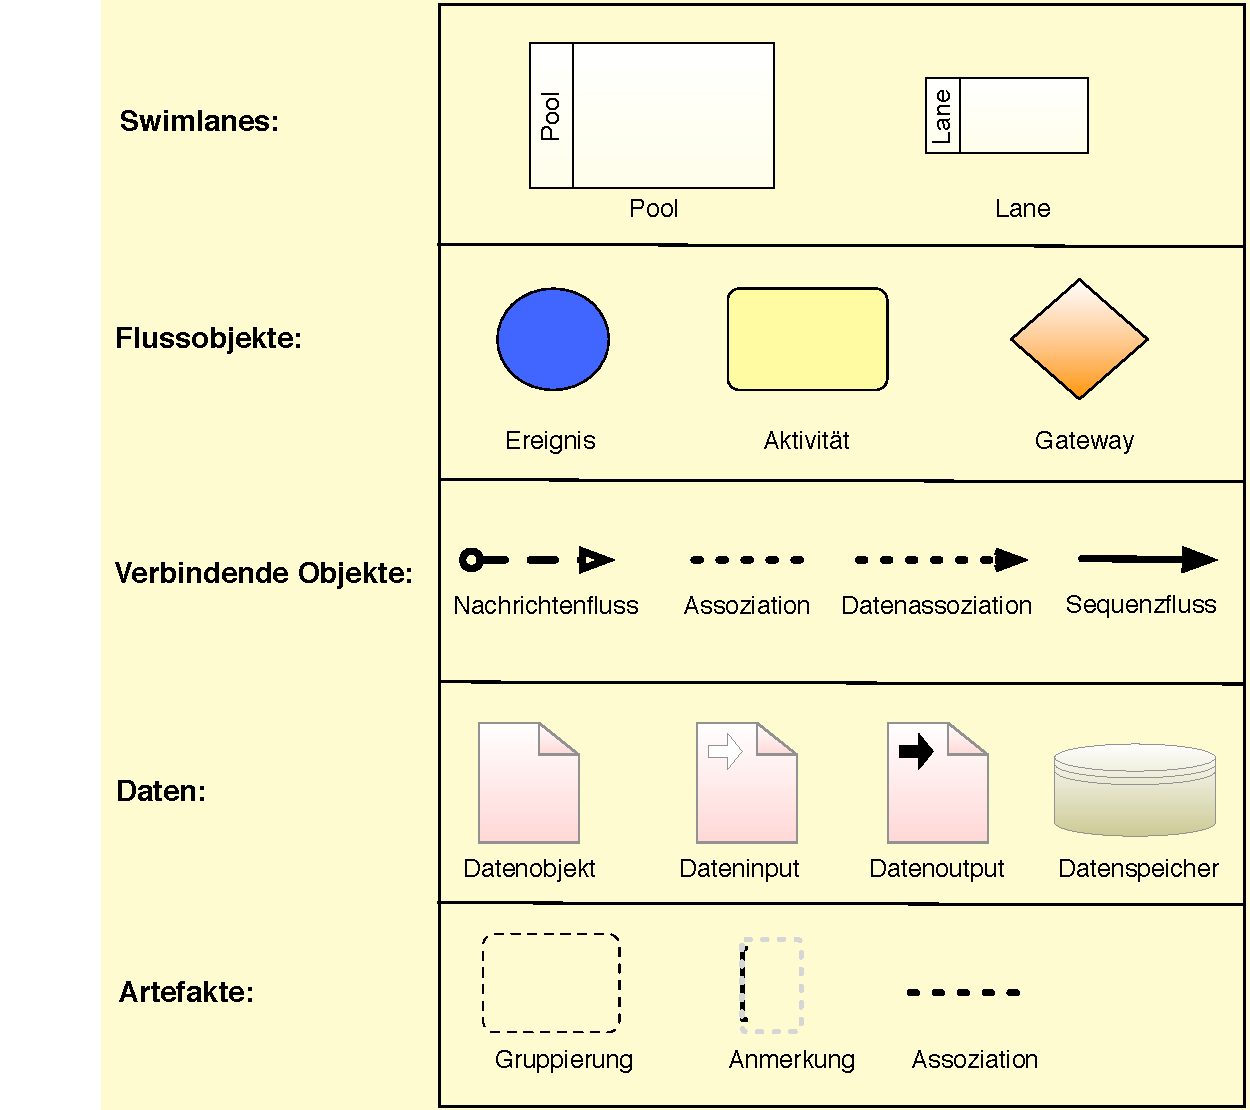
\includegraphics[scale=0.6]{BPMN} %pdf, jpg, png...
  \caption{BPMN-Elemente Übersicht nach \cite{gpfert2012}}
  \label{fig:BPMN}
\end{center}
\end{figure}
In der Kategorie \textbf{Swimlanes} befinden sich \textit{Pools} und \textit{Lanes}. \textit{Pools} stellen eine Art Container für den Prozess dar. Ein \textit{Pool} stellt einen Prozessteilnehmer dar. Ein Prozessteilnehmer ist z.B. eine Organisationseinheit oder eine selbstständige Geschäftseinheit. Werden in einem Prozessmodell mehrere \textit{Pools} verwendet, so können hiermit Kollaborationen zwischen verschiedenen Prozessteilnehmern dargestellt werden. Ein \textit{Pool} kann in mehrere \textit{Lanes} unterteilt werden. \textit{Lanes} können untergeordnete Organisationseinheiten, Partnerrollen (z.B. Vertrieb, Projektleitung, Marketing), oder auch verschiedene Bestandteile eines Systems sein \cite{gpfert2012, pitschke2010, allweyer2013}. \newline
\textit{Aktivitäten}, \textit{Ereignisse} und \textit{Gateways} befinden sich in der Kategorie \textbf{Flussobjekte}.
Start und Ende von Prozessen werden in BPMN durch \textit{Ereignisse} beschrieben. Diese werden in  \textit{Startereignisse} und \textit{Endereignisse} unterschieden.  Weiterhin gibt es auch noch \textit{Zwischenereignisse}. \newline

\textit{Aktivitäten} stellen Arbeitseinheiten dar und stellen einen Oberbegriff für Aufgaben, Unterprozesse und Aufruf-Aktivitäten dar. Beschriftet werden sie mit einer Objekt-Verb-Verbindung (z.B. Lieferung überprüfen) \cite{gpfert2012}. \newline
Mit Hilfe von \textit{Gateways} lässt sich der Prozessablauf kontrollieren und steuern, da durch diese Verzweigungen und Zusammenführungen von Sequenzflüssen dargestellt werden. \cite{gpfert2012, allweyer2013}. Hierbei werden \textit{Exklusive Gateways} zur Modellierung alternativer Pfade, \textit{Parallele Gateways} zur Modellierung parallel ablaufender Pfade, \textit{Inklusive Gateways} zur Modellierung der Auswahl eines oder mehrerer Pfade und \textit{Komplexe Gateways} zur Modellierung komplexer Regeln bei Verzweigungen und Zusammenführungen, unterschieden \cite{allweyer2013}.\newline 

\begin{figure}[H]
\begin{center}
  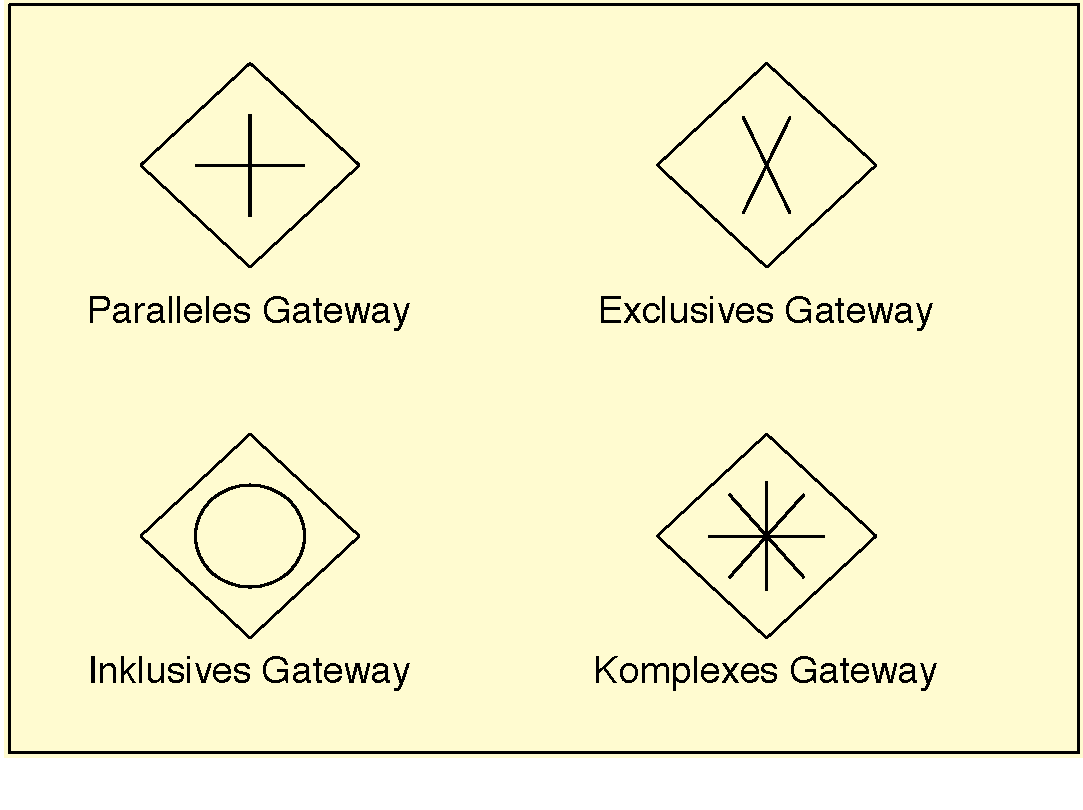
\includegraphics[scale=0.3]{gates} %pdf, jpg, png...
  \caption{BPMN-Gateways}
  \label{fig:gates}
\end{center}
\end{figure} 


\textit{Nachrichtenfluss}, \textit{Assoziation}, \textit{Datenassoziation} und \textit{Sequenzfluss} bilden zusammen die Kategorie \textbf{Verbindende Objekte}. Ein \textit{Sequenzfluss} dient dazu die Reihenfolge der Aktivitäten im Prozess darzustellen. Ein \textit{Nachrichtenfluss} wird dazu verwendet, den Nachrichtenfluss zwischen zwei getrennten Prozessteilnehmern, z.B. aus zwei verschiedenen Unternehmen, darzustellen. Mit Hilfe einer \textit{Assoziation} können Daten-, Text und andere Artefakte mit Flussobjekten verknüpft werden. Hiermit werden die In- und Outputs von Aktivitäten aufgezeigt \cite{white2004}. \newline
In der Kategorie \textbf{Daten} befinden sich \textit{Datenobjekte}, \textit{DatenInput}, \textit{DatenOutput} und \textit{Datenspeicher}. \textit{Datenobjekte} geben hierbei an, welche Daten von den Aktivitäten benötigt werden, bzw. von diesen erzeugt werden \cite{white2004}. Sie stellen somit Information dar, welche durch den Prozess fließen. Bei einem  \textit{DatenInput} Handelt es sich um einen externen Input für den ganzen Prozess, der von einer Aktivität gelesen wird. Ein \textit{DatenOutput} hingegen wird als Ergebnis eines ganzen Prozesses erzeugt. Somit handelt es sich bei \textit{DatenInput}, bzw. \textit{DatenOutput} um Eingangs-, bzw. Ausgangsprozessschnittstellen \cite{bpmnposter}. Ein Datenspeicher kann für den indirekten Austausch von Daten zwischen zwei verschiedenen Prozessteilnehmern verwendet werden. Hierfür ist es notwendig, dass beide Prozessteilnehmer Zugriff auf den Datenspeicher haben \cite{allweyer2013}.
Die Kategorie \textbf{Artefakte} beinhaltet \textit{Gruppierung}, \textit{Anmerkung} und \textit{Assoziation}.  Diese ergänzen den Prozess um zusätzliche Informationen, haben jedoch keinerlei Einfluss auf diesen \cite{gpfert2012}. Eine \textit{Gruppierung} kann hierbei zur Dokumentation oder für Analysezwecke benutzt werden. Durch eine \textit{Annotation} können dem Leser zusätzliche Informationen in Textform bereit gestellt werden \cite{white2004}.




\subsection{Deklarative Modellierung}

 Die deklarative Modellierung folgt im Gegensatz zur imperativen Modellierung einem \grqq Outside-In-Ansatz\grqq  \cite{lichtenegger2012}. Deklarative Sprachen legen den Ablauf nicht im Vorhinein fest. \cite{pichler2012}. Sie sind somit sehr flexibel \cite{reichert2012}. Zu Beginn befinden sich nur die Aktivitäten im Prozessmodell und erlauben jegliches Ausführungsverhalten. Erst wenn Constraints zum Modell hinzugefügt werden, werden schrittweise Ausführungsalternativen verworfen \cite{pichler2012}. Constraints lassen sich hierbei in die beiden verschiedenen Kategorien \textbf{Ausführungsconstraints} und \textbf{Terminierungsconstraints} einteilen. Die Ausführungsconstraints geben Einschränkungen für die Ausführung von Aktivitäten an. Hierbei kann es sich z.B. um die Anzahl möglicher Ausführungen oder eine Mindestzeitverzögerung zwischen zwei Aktivitäten handeln. Terminierungsconstraints hingegen geben an, wann eine korrekte Terminierung möglich ist. Z.B. kann hier vorgeschrieben werden, dass eine Aktivität mindestens einmal ausgeführt werden muss oder dass der Aktivität A Aktivität B folgen muss \cite{reichert2012}.  Abbildung \ref{fig:Dec} zeigt ein Beispiel für ein deklaratives Prozessmodell. Es besteht aus den drei Aktivitäten A,B und C sowie aus zwei Constraints: Das Constraint bei Aktivität C legt fest, dass diese mindestens einmal ausgeführt werden muss, aber beliebig oft ausgeführt werden kann und das Constraint zwischen A und B legt fest, dass Aktivität B Aktivität A vorausgehen muss. Abgesehen von diesen Bedingungen, können die Aktivitäten sowohl beliebig oft, als auch in beliebiger Reihenfolge ausgeführt werden.

\begin{figure}[H]
\begin{center}
  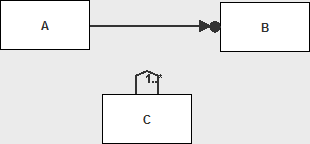
\includegraphics[scale=0.6]{DecProcessModel} %pdf, jpg, png...
  \caption{Deklarativer Beispiel-Prozess}
  \label{fig:Dec}
\end{center}
\end{figure} 

\subsubsection{ConDec}

Die deklarative Modellierungssprache ConDec wurde erstmals unter dem Namen DecSerFlow veröffentlicht \cite{fahland2010}. Mit ConDec lassen sich einerseits sehr strenge Modelle erstellen, welche den gesamten Prozess im Detail vorgeben und andererseits sehr leichte Modelle, welche zwar vorgeben, welche Arbeit getan werden muss, aber nicht wie sie getan werden muss \cite{pesic2006}. \newline
In ConDec gibt es die vier verschiedenen Contraints \textit{Existence}, \textit{Choice}, \textit{Relation} und \textit{Negation}. Tabelle \ref{tab:tab3} zeigt die Bedeutung der verschiedenen Constraints. \newline

\begin{table}
\begin{tabular}{|p{0.5\textwidth}|p{0.5\textwidth}|}
\hline
\textbf{Constraint} & \textbf{Erläuterung}\\
\hline
Existente Constraints & Ein-stellige Kardinalitäts-Constraints. Sie geben an wie oft eine Aktivität ausgeführt werden kann, bzw. muss.\\
\hline
Choice Constraints & N-stellige Constraints. Sie geben die Notwendigkeit der Ausführung von Aktivitäten an, die zu einer Reihe möglicher Alternativen gehören, unabhängig von anderen Constraints. \\
\hline
Relation Constraints & Zwei-stellige Constraints. Sie geben vor, dass eine gewisse Aktivität ausgeführt werden muss, falls eine andere Aktivitäten ausgeführt wird. Es können auch qualitative zeitliche Constraints zwischen diesen beiden Aktivitäten verlangt werden.\\
\hline
Negation Constraints & Stellt die negative Version der Relation Constraints dar. Sie verbieten explizit die Ausführung einer gewissen Aktivität, wenn eine andere Aktivität ausgeführt wird.\\
\hline
 \end{tabular}
  \caption{Constraints ConDec}
\label{tab:tab3}
 \end{table}
 
 Eine Übersicht über die genaue Notation von ConDec ist in Abhang A verfügbar.
 







